\section{Discount usability evaluation method}
When we are talking about the discount evaluation method, we are talking about the cooperative evaluation created by andrew monk et al. 1993\todo{cite Improving your human-computer interface: A practical technique}. Table ref from the book title\todo{cite} outlines the steps from the method.

\begin{figure}[]
  \centering      
    \begin{subfigure}[b]{\textwidth}
    \begin{center}
      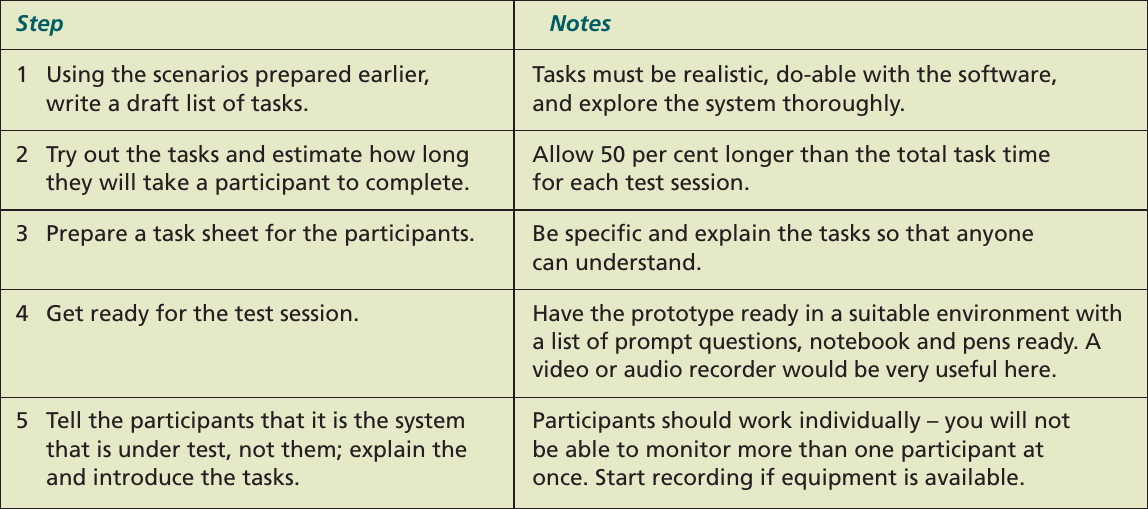
\includegraphics[scale=0.5]{./pics/UsabilityTableP1}
      \caption{table part 1}
      \label{fig:bluej_iterator_code}
    \end{center}
    \end{subfigure}
    ~\\
    \begin{subfigure}[b]{\textwidth}
    \begin{center}
      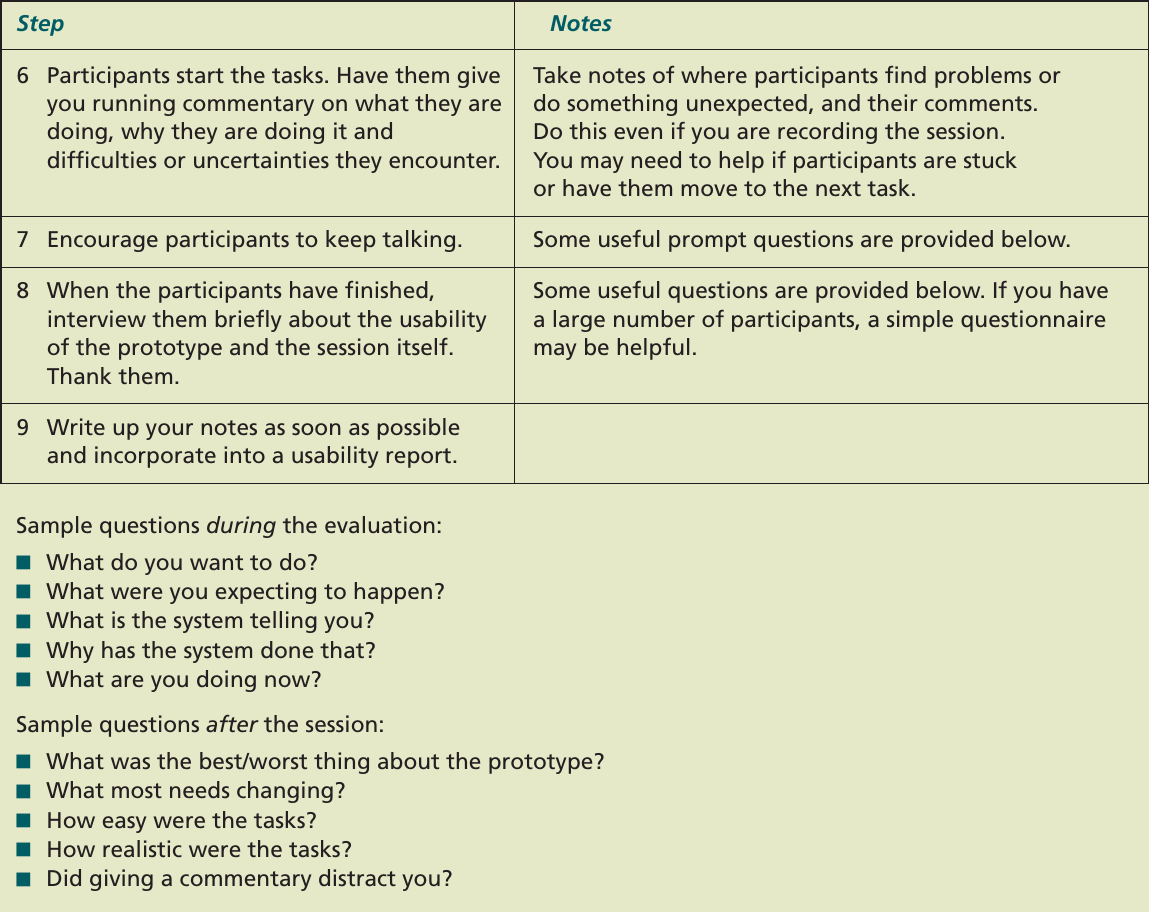
\includegraphics[scale=0.5]{./pics/UsabilityTableP2}
      \caption{table part 2}
      \label{fig:bluej_iterator_code2}
    \end{center}
    \end{subfigure}
    \caption{combined caption}
    \label{fig:bluej_iterator}
\end{figure}

This method is focused on finding the bigger usability problems over finding a lot of them, and has thus proven to be both lightweight and useful. In particular cite shows that you only need about 5 test subjects to get clear feedback on your system. 

https://www.nngroup.com/articles/why-you-only-need-to-test-with-5-users/